%\lstset{language=Pascal}
\section{Ersten Song schreiben}
\label{sec:ErstenSongSchreiben}

Damit wir Musik porten können, benötigen wir zuallererst folgende Programme:
\begin{itemize}
	\item Einen Texteditor unserer Wahl
	\item \href{https://dl.smwcentral.net/24994/AddmusicK_1.0.8.zip}{AddMusicK}, um die zu portierende Textdatei in eine Rom zu patchen und zusätzlich eine SPC Datei zu kompilieren.
	\item Einen SPC Player (am besten \href{https://dl.smwcentral.net/15205/SPC700\%20PLAYER.zip}{SPC700 Player}) zum abspielen von SPC Dateien.
\end{itemize}

In späteren Kapiteln werden noch weitere Programme benötigt.

\bigskip

Ein Song ist in 2 Teile aufgeteilt. Im ersten Bereich werden hauptsächlich Instrumente und Makros definiert. Alle Befehle die sich hier befinden sind so genannte Spezial Befehle (beginnen mit \# -- nicht zu verwechseln mit einem Kanal) und einige wenige Standard Befehle. Im zweiten Bereich befinden sich die Kanäle, die mit Noten und Hex-, sowie Standard Befehlen gefüllt sind.

\subsection{Standard- und Spezialbefehle}

Wir fangen nun ein neues Textdokument an. Wo sich dieses befindet ist egal, ich empfehle einen neuen Ordner custom anzulegen unter AddMusicK/music/ der neben dem Ordner originals liegt. Unser erster Song wird das populäre Prelude aus der Final Fantasy Reihe werden. Der Song soll parallel zu diesem Tutorial selbst geschrieben werden.

\bigskip

Damit wir ein Song porten können, muss dieser nur die zwei folgenden Dinge besitzen:
\begin{itemize}
	\item Den Spezial Befehl \#amk 2 -- die 2 gibt an, welchen Song Parser AddMusicK benutzen soll. Dieser Wert kann sich mit einer neueren Version von AddMusicK ändern. AddMusicK schreibt den Befehl entweder am Anfang oder am Ende des Dokumentes auch selbstständig hin, falls der Befehl nicht im Textdokument steht.
	\item Den 1. Kanal, Kanal \#0
\end{itemize}

\subsubsection{Tempo und Lautstärke}
Mit dem Standard Befehl t geben wir das Tempo an. Dieses wird nicht wie üblich in BPM (Beats per Minute, also Viertelnoten pro Minute) angegeben, lässt sich aber wie folgt umrechnen: $ BPM \cdot 0,4096 = t \, Wert $ \\
Unser Song besitzt einen BPM Wert von 78. Daraus wird also 31,9488. Weil nur Integer Werte (ganze Zahlen) verwendet werden können, runden wir das Tempo auf t32 auf.

\bigskip

Mit dem Standard Befehl w geben wir die globale Lautstärke des Songs an. Der Wertebereich liegt bei w0 bis w255. Wir legen diesen auf w180. Wird kein w Wert festgelegt, wird er von AddMusicK auf w200 gesetzt. Beide Befehle müssen sich entweder über dem 1. Kanal oder direkt am Anfang des 1. Kanals befinden.

\bigskip

Im folgenden Bild ist eine so genannte Piano Roll zu sehen. Die höchste Note ist ein o8c, was zu hoch für die Rahmenbedingung ist. Wie vorher erwähnt ist unsere absolute Oktavenhöhe für die maximale Tonhöhe aber nebensächlich. Daher verschieben wir gedanklich alle Noten um 2 Oktaven nach unten. Somit beginnt die erste Note im zweiten Oktavenraum. 

\begin{figure}[htbp] \centering
	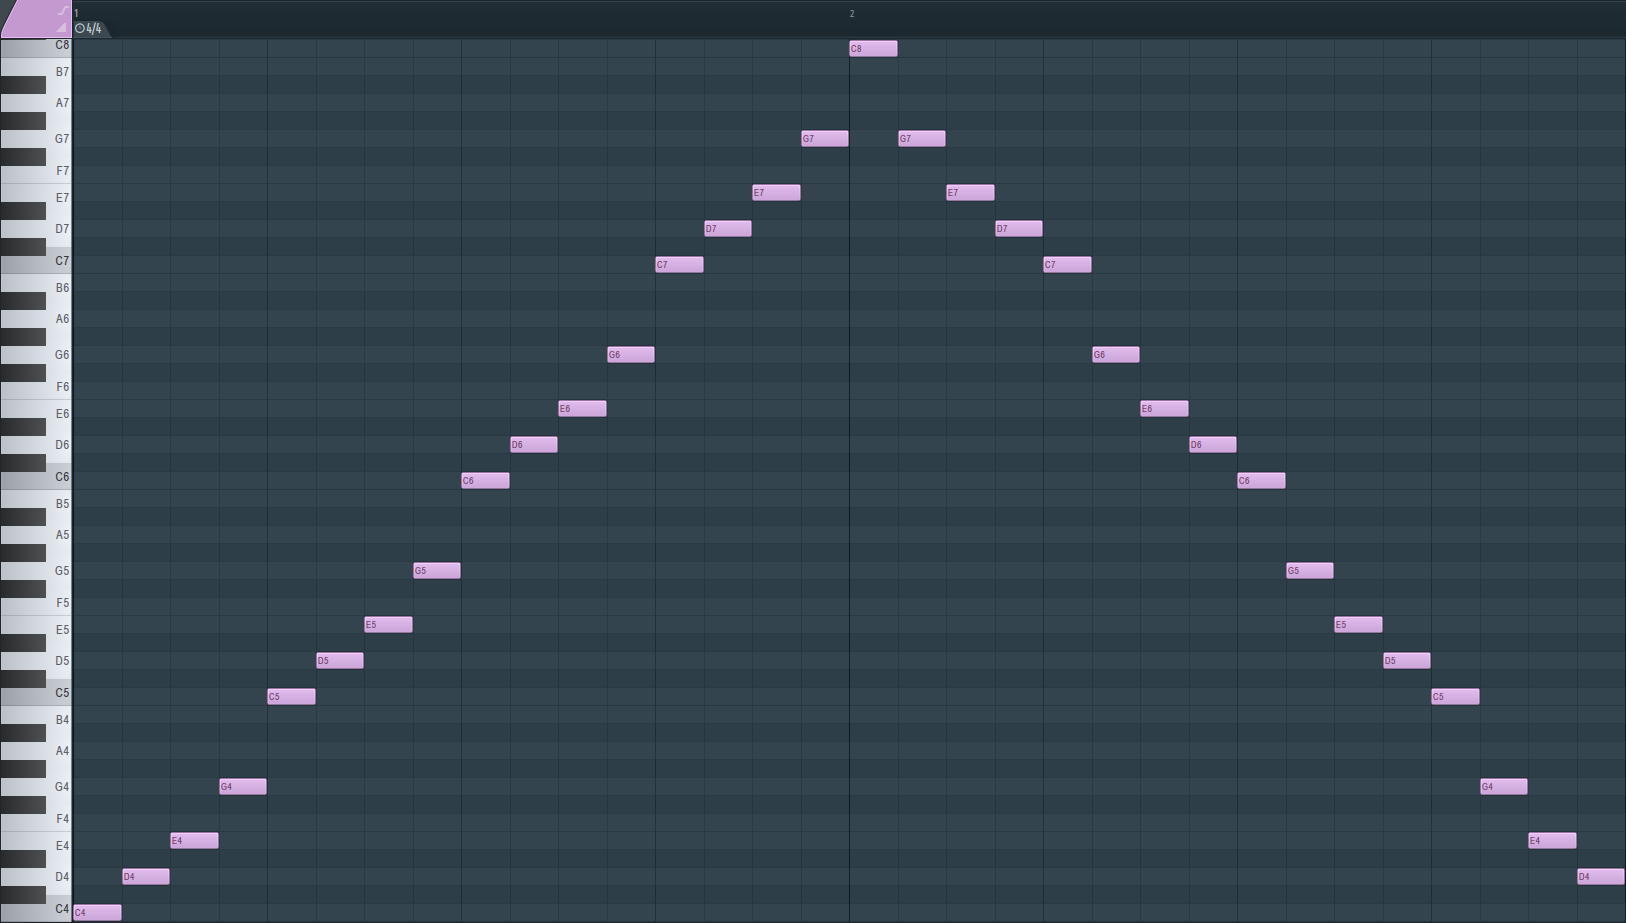
\includegraphics[width=.95\linewidth]{images/Noten_A.png}
	\caption{Notenabfolge A}
	\label{NotenabfolgeA}
\end{figure}
Unser Dokument sieht bisher wie folgt aus:

\medskip

\lstinputlisting[framexleftmargin=8mm, frame=shadowbox, rulesepcolor=\color{blue}, numbers=left]{codes/PreludeKanal1_1.txt}

%\medskip
\clearpage

Wir füllen nun den 1. Kanal mit Noten. Im Bild sehen wir die Noten der ersten 2 Takte (engl. Bar. Ein Takt besteht bei einem 4/4-Takt aus 4 Viertelnoten, bei einem 3/4-Takt aus 3 Viertelnoten usw.) Die einzelnen Noten sind daher 16tel Noten. Die gezeigte Notenfolge nennen wir zur Veranschaulichung A. \\
Nun schreiben wir die Noten in den Kanal: c16 d16 e16 g16

\bigskip

Ein Wechsel in einen anderen Oktavraum können wir entweder durch erneutes setzen des o Befehls erreichen oder durch > (Wechsel in den nächst höheren Raum) bzw < (Wechsel in den nächst niedrigeren Raum). Die bevorzugte Variante sollte > und < sein. Der Vorteil liegt darin, dass > und < den Oktavraum in Relation zum vorherigen angeben, während der o Befehl einen absoluten Wert festlegt. Durch das Ändern der ersten Oktave eines Kanals bewegen sich daher alle Noten mit dem gleichen Oktavabstand mit, während bei der Nutzung von o Befehlen jede Oktave manuell geändert werden müsste. \\
Für die ersten zwei Takte ergibt sich dadurch:

\medskip

\lstinputlisting[framexleftmargin=8mm, frame=shadowbox, rulesepcolor=\color{blue}, numbers=left]{codes/PreludeKanal1_2.txt}

\medskip

Leerzeichen und Zeilenumbrüche werden von AddMusicK nicht interpretiert und dienen nur der besseren Übersicht.
Mit einem Semikolon ; können Kommentare eingefügt werden. Ein Kommentar wird von AddMusicK vollständig ignoriert und nimmt keinen Platz im Arbeistspeicher ein.

\subsubsection{Standardlänge}

Mit dem l Befehl (length) kann die Standardlänge von Noten und Pausen definiert werden, also der Länge, die von AddMusicK angenommen wird, wenn keine Länge hinter einer Note bzw. Pause steht (normalerweise 1). Da alle Noten in diesem Kanal aus 16tel Noten bestehen, können wir den Code mit l16 übersichtlicher gestalten. Hierbei sei gesagt, dass der l Befehl nicht die Größe des Songs verringert, sondern nur der Übersicht dient. Das Textdokument sieht nun folgendermaßen aus:

%\medskip
\clearpage

\lstinputlisting[framexleftmargin=8mm, frame=shadowbox, rulesepcolor=\color{blue}, numbers=left]{codes/PreludeKanal1_3.txt}

\medskip

Im folgenden Bild sehen wir die Noten der nächsten 2 Takte. Die Notenabfolge nennen wir B. Zu Übungszwecken soll diese selbst geschrieben werden.

%\newpage

\begin{figure}[htbp] \centering
	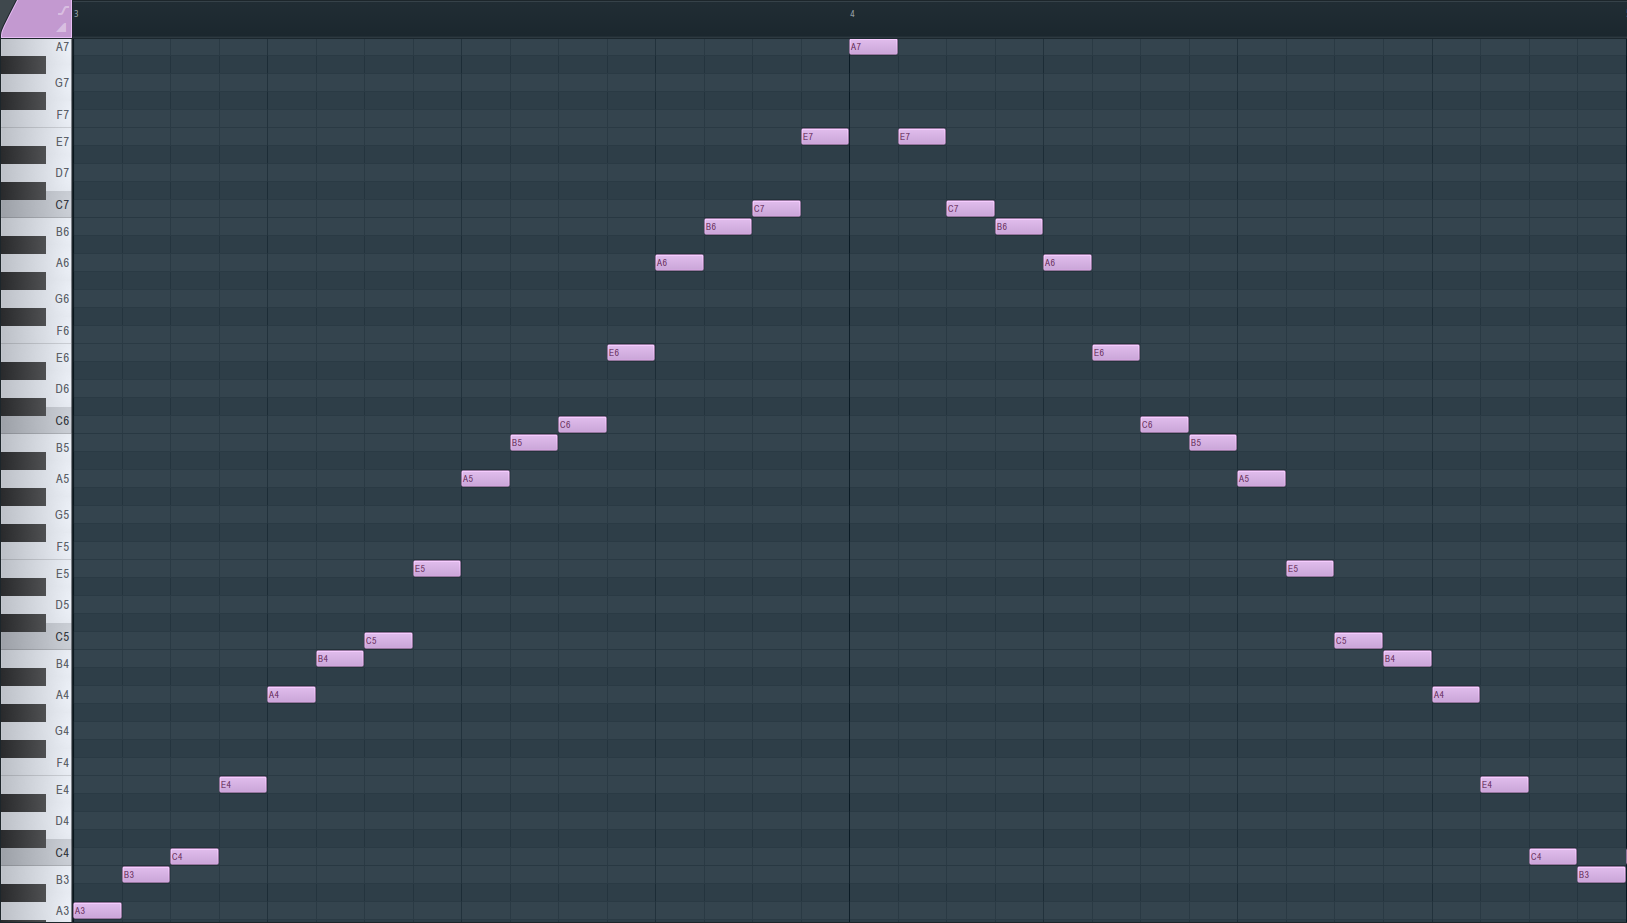
\includegraphics[width=.95\linewidth]{images/Noten_B.png}
	\caption{Notenabfolge B}
	\label{NotenabfolgeB}
\end{figure}

Wenn alles geklappt hat, sieht der Song nun wie folgt aus:

\medskip

\lstinputlisting[framexleftmargin=8mm, frame=shadowbox, rulesepcolor=\color{blue}, numbers=left]{codes/PreludeKanal1_4.txt}

\medskip

Dies ist eine gute Gelegenheit, um den Song Probe zu hören.
Dafür öffnen wir \textit{AMKGUI.exe}, scrollen im unteren Fenster Local Songs so weit nach unten wie es geht und klicken auf den letzten Song. Als nächstes gehen wir auf \textit{Add new Song} und wählen unsere Textdatei aus. Diese sollte jetzt markiert sein. Als nächstes setzen wir den Haken bei \textit{Porter mode} und klicken auf \textit{Run}. AddMusicK erzeugt aus der Textdatei eine SPC Datei die automatisch abgespielt wird, sofern der SPC Player als Standardprogramm für SPC Dateien gesetzt wurde. Falls dies nicht der Fall ist, wird eine Fehlermeldung erscheinen und wir müssen die SPC manuell öffnen. Eine SPC Datei wird nach dem Porten automatisch im Ordner SPCs abgelegt.


\begin{figure}[htbp] \centering
	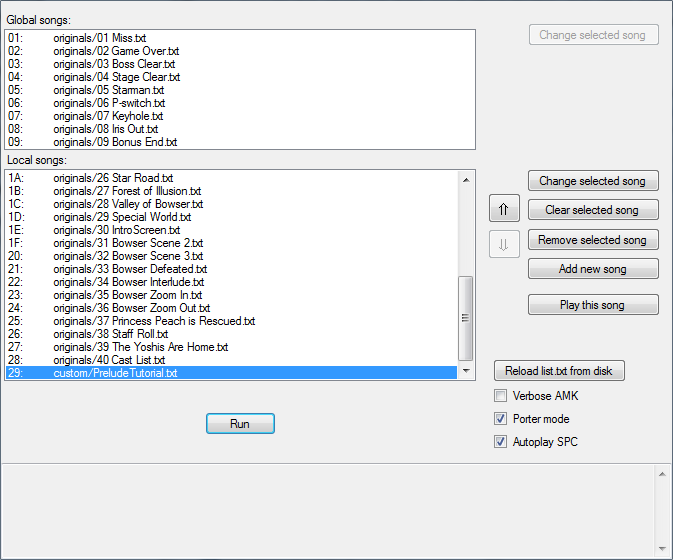
\includegraphics[width=.95\linewidth]{images/AMKGUI.png}
	\caption{AMKGUI.exe}
	\label{AMKGUI}
\end{figure}


Als nächstes kommen wieder Notenfolge A und B. Anstatt die Notenfolgen zu kopieren, benutzen wir ein neues Werkzeug und zwar Loops.

\subsubsection{Loops}
Jede Note die wir schreiben vergrößert den Song. Mit Loops können wir wiederkehrende Notenabfolgen zusammenfassen, einmalig speichern und aufrufen wann wir wollen.
Das Speichern eines Loops verbraucht zwar ebenso Speicherplatz, ist der Loop aber groß genug und wird mehrfach aufgerufen, kann man dadurch eine Menge Platz im Arbeitsspeicher sparen.
Hierbei sei gesagt, dass man auf keinen Fall extrem kurze oder gar nur einzelne Noten in einen Loop speichern sollte, weil dies den umgekehrten Effekt hat und den Song vergrößert. \\
Es gibt 3 Arten von Loops: Normale Loops, Labeled Loops und Superloops. Wir verwenden hier einen normalen Loop. Dieser speichert alles was sich in eckigen Klammern [] befindet in einem Loop ab, eine Zahl dahinter gibt an, wie oft dieser Loop gespielt werden soll. Unsere Notenabfolge A B A B wird dadurch zu [A B]2


\lstinputlisting[framexleftmargin=8mm, frame=shadowbox, rulesepcolor=\color{blue}, numbers=left]{codes/PreludeKanal1_5.txt}

\medskip

Wichtig bei Loops im allgemeinen ist folgendes zu beachten: Ein sauberer normaler Loop hat immer gleich viele > und <. Dadurch ist sichergestellt, dass wir uns am Ende eines Loops in der gleichen Oktave befinden wie am Anfang des Loops. Ist dies nicht der Fall, laufen die Noten beim erneuten Durchlauf aus. Daher muss wie im Codebeispiel am Ende der Notenabfolge B ein > platziert werden.
Täten wir dies nicht, würde beim zweiten Durchlauf des Loops das erste C nicht in der zweiten Oktave beginnen, sondern in der ersten, weil das die letzte Oktave war in der wir uns befanden als das letzte B gespielt wurde.

\bigskip

Als nächstes kommen die Notenabfolgen C, D, E und F. Wer mag, kann diese zu Übungszwecken selbst schreiben, die Bilder dazu befinden sich im Anhang.

Der Song sieht nun wie folgt aus:

%\newpage
\medskip

\lstinputlisting[framexleftmargin=8mm, frame=shadowbox, rulesepcolor=\color{blue}, numbers=left]{codes/PreludeKanal1_6.txt}

\medskip

Diese gesamte Notenabfolge A B A B C D E F bzw. [A B]2 C D E F wird 3 mal hintereinander abgespielt. Es bietet sich daher an, einen weiteren Loop zu verwenden. Einen normalen Loop können wir aber nicht in einen anderen normalen Loop verschachteln. Dafür gibt es Superloops, gekennzeichnet durch doppelte Eckige Klammern [[]].
Dadurch wird unser Song zu [[ [A B]2 C D E F ]]3. \\
In eine weitere Ebene zu verschachteln ist nicht möglich, es können jedoch beliebig viele normale und labeled Loops parallel in einem Superloop zusammengefasst werden. \\
Nachdem der Superloop platziert wurde, sieht unser Song wie folgt aus:

\medskip

\lstinputlisting[framexleftmargin=8mm, frame=shadowbox, rulesepcolor=\color{blue}, numbers=left]{codes/PreludeKanal1_7.txt}

\medskip

Alle Noten für Kanal \#0 sind gesetzt. Wir können diesen Kanal nun weiter bearbeiten.

\subsubsection{Panning}
Panning (oder kurz Pan) bezeichnet die Aufteilung der Lautstärke auf unterschiedliche Lautsprecher. Der entsprechende Befehl in MML ist y. Gültige Werte liegen zwischen 0 und 20, dabei gilt: \\
y0 : 100\% Lautstärke auf rechten Lautsprecher \\
y20 : 100\% Lautstärke auf linken Lautsprecher \\
y10 : 50\% Lautstärke auf rechten und linken Lautsprecher (Standardwert) 

\bigskip

Panning hilft uns dabei, einen Song räumlicher klingen zu lassen. \\
Es ist auch möglich, Panning kontinuierlich zu ändern. Dafür verwenden wir unseren ersten Hex-Befehl.

\bigskip
Hex-Befehle erkennt man daran, dass diese immer mit einem \$ beginnen, gefolgt von einem zweistelligen Hexwert. Der Befehl für das so genannte Pan Fading ist \$DC \$XX \$YY, wobei XX und YY Hexwerte sind, die das Fading weiter beschreiben. \$XX gibt die Dauer des Prozesses an, \$YY gibt den Panning Wert an, auf den geändert werden soll. \\
Wir möchten in Kanal \#0 das Panning so haben, dass es mit 75\% links und 25\% rechts beginnt (y15) und nach einem Takt mit 75\% rechts und 25\% links aufhört (y5). Danach soll das Panning für den nächsten Takt den genau entgegengesetzten Verlauf haben, sodass wir nach insgesamt 2 Takten wieder bei y15 sind. Dieser Vorgang soll sich in Kanal \#0 durch den gesamten Song ziehen. \\
Als erstes müssen wir unseren Startwert festlegen, also y15. Danach kommt der erste Hexbefehl \$DC. Als nächstes kommt die Dauer. 1 Takt bzw. eine ganze Note als Hexwert ausgedrüct ist \$C0. Diesen Wert kann man entweder ausrechnen (siehe Ticks) oder in der entsprechenden Tabelle im Anhang nachschauen. Unser Zielwert ist 5.  Der erste Befehl um die Lautstärke vom linken zum rechten Lautsprecher zu verschieben ist somit fertig definiert:  \$DC \$C0 \$05.\\
Wollen wir wieder auf y15 zurück, machen wir dies mit \$DC \$C0 \$0F, wobei 15 als Hexwert \$0F ist. Wer Probleme beim Umrechnen von Dezimalzahlen zu Hexwerten hat kann auch einen Taschenrechner benutzen und diesen auf Programmierer einstellen.
Die beiden Befehle schreiben wir nun abwechselnd nach jeweils einem Takt in den ersten Kanal. \\
Der Song sollte nun folgendermaßen aussehen:

\medskip

\lstinputlisting[framexleftmargin=8mm, frame=shadowbox, rulesepcolor=\color{blue}, numbers=left]{codes/Panning.txt}

\medskip

\subsubsection{Instrumente setzen}
Instrumente werden mit @ ausgewählt, gefolgt von einer Nummer. Mit 0 - 18 und 21 - 29 werden Instrumente bestehend aus Super Mario World Samples mit bestimmten Voreinstellungen angewählt. Instrumentnummern 30+ sind Instrumente, die in \#instruments definiert wurden. Dabei ist es egal, ob die dafür verwendeten Samples aus SMW kommen oder eigene -- sogenannte custom Samples -- verwendet werden. Das Standardinstrument ist @0 was automatisch gewählt wird, wenn in einem Kanal kein Instrument platziert wird.
Eine vollständige Liste der SMW Samples befindet sich im Anhang. \\
Zum Testen empfehle ich in Zeile 7 verschiedene Instrumente auszuwählen, z.B. @2, @3 oder @5 und diese anzuhören. \\
Das Sample des Standardinstruments @0 soll beibehalten werden, allerdings ändern wir dessen ADSR Werte (Attack, Decay, Sustain, Release). Dafür gibt es zwei Möglichkeiten. Entweder mit dem Hex-Befehl \$ED oder mit dem Spezial Befehl \#instruments. Wir verwenden letzteres, die genaue Funktionsweise und Unterschiede werden im Kapitel ADSR weiter erläutert.

\bigskip

Wir definieren uns nun ein neues Instrument auf Basis des Samples von @0 mit anderen Eigenschaften.
Da es sich hierbei um einen Spezial Befehl handelt, kommt dieser in den ersten Teil des Dokuments. Das neu definierte Instrument rufen wir mit @30 auf.

\medskip

\lstinputlisting[framexleftmargin=8mm, frame=shadowbox, rulesepcolor=\color{blue}, numbers=left, lastline=12]{codes/Instrument30.txt}

\medskip

Wir bauen unseren Song nun weiter. Im Folgenden Bild sehen wir einige Begleitakkorde. 

\begin{figure}[htbp] \centering
	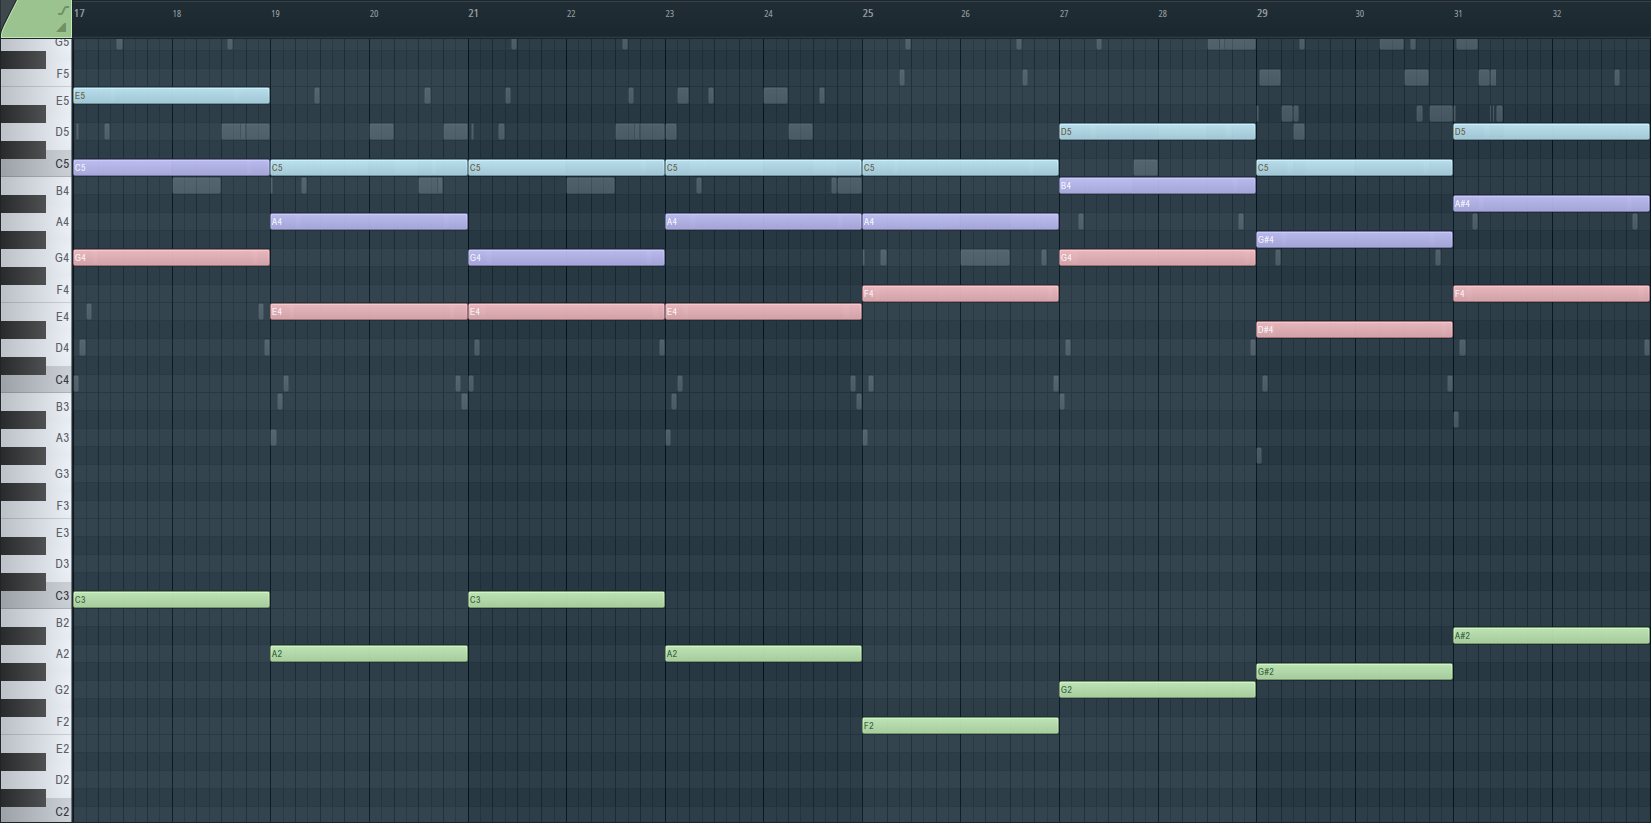
\includegraphics[width=.95\linewidth]{images/Strings.png}
	\caption{Kanal 2 bis 5}
	\label{NStrings}
\end{figure}

Der erste Kanal ist vollständig und wird nicht weiter bearbeitet. Parallel zum 1. Kanal folgt nach 16 Takten eine Begleitung. Die Noten erstrecken sich jeweils über 2 Takte und haben deshalb einen Notenwert
von 1\textasciicircum1. Pro Kanal kann aber nur eine Note gleichzeitig platziert werden. Deshalb brauchen wir für diese Begleitung 4 Kanäle. Die Noten ordnen wir auf die Kanäle wie folgt zu:

\bigskip

Kanal \#1 blaue Noten, angefangen bei Oktave 5 \\
Kanal \#2 lila Noten, angefangen bei Oktave 5 \\
Kanal \#3 rote Noten, angefangen bei Oktave 4 \\
Kanal \#4 grüne Noten, angefangen bei Oktave 3

\bigskip

Die Begleitung soll außerdem ein weiteres mal wiederholt werden, sodass sie von Takt 17 bis 32 und dann nochmal von Takt 33 bis 48 gespielt wird. Zu Übungszwecken sollen diese 4 Kanäle selbst geschrieben werden.

\bigskip

Kanal \#1 bis \#4 sollten wie folgt aussehen: 

\medskip

\lstinputlisting[framexleftmargin=8mm, frame=shadowbox, rulesepcolor=\color{blue}, numbers=left, firstline=41]{codes/Instrument30.txt}

\medskip

Als nächstes definieren wir uns ein neues Instrument auf Basis des Samples von @1 für die vier Kanäle.
Wir fügen es in \#Instruments ein und können es mit @31 auswählen.
Hierbei ist auf die Reihenfolge der Instrumente zu achten, weil diese die Nummerierung vorgibt. Das @30 und @31 hinter den Semikolons sind nur Kommentare.

\medskip

\lstinputlisting[framexleftmargin=8mm, frame=shadowbox, rulesepcolor=\color{blue}, numbers=left, firstline=3, lastline=7]{codes/Instrument31.txt}

\medskip

Wir weisen allen Noten in Kanal \#1, \#2, \#3 und \#4 das neue Instrument mit @31 zu und hören den Song probe. Nach ungefähr 47 Sekunden setzt unsere Begleitung ein.

\subsubsection{Lokale Lautstärke}
Wie wir bereits gelernt haben, wird mit dem w Befehl die globale Lautstärke des Songs eingestellt. Mit dem v Befehl können Noten der einzelnen Kanäle zusätzlich individuell eingestellt werden. Auch hier liegt der Wertebereich zwischen v0 und v255. \\
Die Noten in den vier neuen Kanälen stellen wir etwas leiser ein, indem wir in jeden der Kanäle ein v220 schreiben. Zusätzlich dazu stellen wir das Panning ein, damit die Akkorde ein wenig auf den Lautsprechern aufgeteilt werden. \\
Die Kanäle mit der Begleitung sehen nun so aus: \\

\medskip

\lstinputlisting[framexleftmargin=8mm, frame=shadowbox, rulesepcolor=\color{blue}, numbers=left, firstline=44, lastline=62]{codes/PreludeTutorial.txt}

\medskip

Als letztes fehlt noch ein weiteres Instrument was in Kanal \#5 zum Einsatz kommen soll. Wir definieren es wie folgt:

\medskip

\lstinputlisting[framexleftmargin=8mm, frame=shadowbox, rulesepcolor=\color{blue}, numbers=left, firstline=3, lastline=8]{codes/PreludeTutorial.txt}

\medskip

Da Kanal \#5 extrem kurze Noten enthält die nur schwer ablesbar sind, kann unser letzter Kanal der Vollständigkeit halber einfach aus dem Codebeispiel übernommen werden. \\
Wie wir in Zeile 8 und 9 sehen, kann ein Instrument in einem Kanal beliebig oft gewechselt werden.
Das ist auch notwendig für komplexere Songs um mehr als 8 Instrumente in einem Song benutzen zu können.

\newpage

\lstinputlisting[framexleftmargin=8mm, frame=shadowbox, rulesepcolor=\color{blue}, numbers=left, firstline=64, lastline=73]{codes/PreludeTutorial.txt}

\medskip

An dieser Stelle wird an dem Song nicht mehr weiter geschrieben. Er soll aber dennoch abgespeichert werden, da wir in späteren Kapiteln diesen für andere Beispiele benutzen werden.